\documentclass{article}
\usepackage{tikz, comment}
\usepackage{pifont}
\usepackage{fontspec}
\usetikzlibrary{arrows, decorations.markings, decorations.pathreplacing}
\begin{comment}
:Title: Not defined yet
:Slug: No name yet

Description Here.........
\end{comment}
\begin{document}\centering 

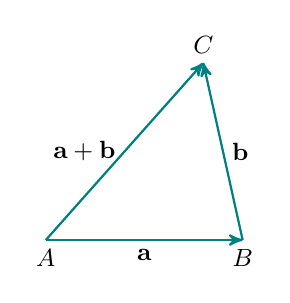
\begin{tikzpicture}[>=latex,xscale=.5*5, yscale=.5*5][font=\sf\small] 

%\draw[xstep=1cm,ystep=1cm,color=gray!80] (-1, -1) grid (4, 5);

\draw[teal, thick, ->, >=stealth'] (0,0)node[black, below]{$A$}
--(1, 0)node[black, below]{$B$};
\node[below, scale=1] at ({1/2}, 0) {$\bf a$};

\draw[teal, thick, ->, >=stealth'] (1, 0)--(0.8, 0.9)node[black, above]{$C$};
\node[right, scale=1] at (0.9, {0.9/2}) {$\bf b$};

\draw[teal, thick, ->, >=stealth'] (0, 0)--(0.8, 0.9);
\node[left, scale=1] at (0.4, {0.9/2}) {$\bf a+b$};

\end{tikzpicture}
\end{document}